\chapter{Continuous Integration}
Continuous Integration is geregeld door Jenkins, dit is een self-hosted omgeving voor continious integration.
Omdat het project met Maven is gebouwd is het makkelijk om CI ondersteuning toe te voegen.
Het commando "mvn test" draait alle tests in het project, als er iets fout gaat is dit ook meteen in Jenkins zichtbaar.

\begin{figure}[H]
	\centering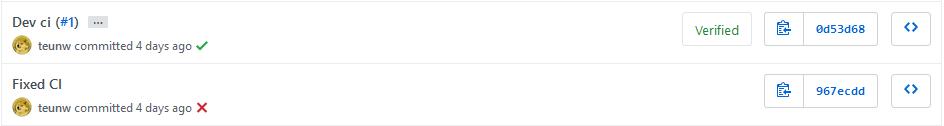
\includegraphics[width=0.35\textwidth]{images/TravisCI.png}
	\caption{Overzicht Jenkins builds}
	\label{fig:jenkins-commits}
\end{figure}
Jenkins wordt geconfigureerd binnen de applicatie zelf, in deze veranderingen staan nu de commando's en Git repoistory geconfigureerd.
Deze configuratie pullt de code vanuit de repository en voert vervolgens het commando "mvn test" uit.
\par
Het bovenstaande script zorgt ervoor dat maven tests automatisch worden uitgevoerd.
De uitslag van deze test is zichtbaar in het build overzicht, zoals in \cref{fig:jenkins-commits} te zien is. Mocht er een build niet succesvol zijn, dan is dit te zien met een rood bolletjes i.p.v. een blauwe.
Jenkins draait je scripts periodiek elke dag, en het resultaat is binnen een paar minuten zichtbaar.

\section{Artifactory}
Nadat Jenkins een build heeft gemaakt wordt deze doorgevoerd naar Artifactory, hier kan de build worden gedownload en ook gedeployed worden op de applicatie server.
Het deployen gebeurt door het WAR bestand weg te schrijven naar een map op de applicatieserver, deze pakt deze vervolgens op en deployed deze.
\begin{figure}[H]
	\centering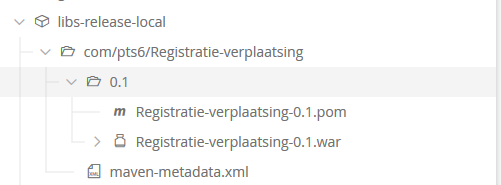
\includegraphics[width=0.6\textwidth]{images/Artifactory_Builds.png}
\end{figure}

\section{Deployment naar TAP omgevingen}
Het bouwen van de applicaties en het automatisch testen van deze applicaties wordt uitgevoerd in de ontwikkel omgeving. Jenkins is geconfigureerd dat wanneer een applicatie gebouwd is, deze automatisch gedeployed wordt naar de juiste applicatie server.
\newline
Zoals in hoofstuk 5.1 te lezen is, wordt na het succesvol bouwen van de applicatie deze gearchiveerd in Artifactory. Hierdoor is het mogelijk om bijvoorbeeld vanuit een shell-script een bepaalde versie van de applicatie op te halen.
\newline
De docker images van de gebruikte applicatie servers zijn uitgebreid met een eigen shell (.sh) script. Door command line toegang te geven tot dit bestand, is het mogelijk om dit uit te voeren.
\subsection{Inhoud shell script}
Het zelf ontwikkelde shell script is beschikbaar op de applicatie servers die gebruikt worden. Hierdoor heeft het shell script toegang tot de deployment folder van de applicatie server. Dit stelt ons in staat om vanuit Artifactory de gewenste versie van een applicatie te downloaden en deze in de deployment folder te plaatsen. Onderstaande stappen geven de werking van het shell script correct weer:
\begin{itemize}
	\setlength\itemsep{0em}
	\item Connectie maken met applicatie server (via Command Line Interface)
	\item deploy-\{applicatie-naam\}.sh aanroepen met bestandsnaam als parameter
	\item Deploy script gaat naar juiste deployment folder van applicatie server
	\item Deploy script download gewenste versie van applicatie naar deployment folder
	\item Applicatie server ziet te wijzigingen en probeert de applicatie te deployen
\end{itemize}
Onderstaande afbeelding geeft een voorbeeld van de inhoud van het shell script. Hierin is zichtbaar dat de parameter '\$1' wordt gebruikt. Dit is de applicatie naam parameter die gebruikt wordt bij het aanroepen van het shell script.

\begin{figure}[H]
	\centering
	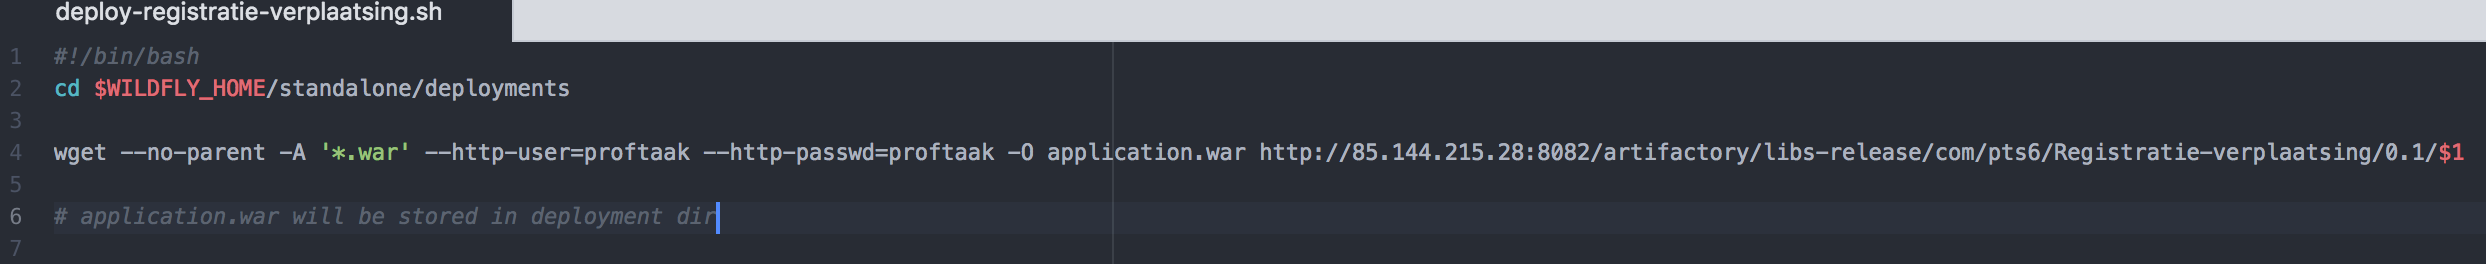
\includegraphics[width=0.95\textwidth]{images/DeploymentScript.png}
	\caption{Voorbeeld shell script voor deployment naar omgeving}
	\label{fig:DeploymentScript}
\end{figure}
Voor elke omgeving van de applicaties die ontwikkeld worden is een apart shell script gemaakt. Dit komt doordat de URL van Artifactory waarin de verschillende applicaties beschikbaar zijn per applicatie anders is. Een verbetering die we hierin kunnen doorvoeren is bijvoorbeeld aan de hand van een extra parameter de juiste URL kiezen voor het downloaden van de applicatie.